\documentclass[a4paper,12pt]{article}
\usepackage{graphicx}
\usepackage{placeins}

\begin{document}

\title{WeatherApp | Documentation}
\author{Vilma Pirilä, Valma Haavisto, Aarni Akkala}

\maketitle

\section{Software Structure}

\subsection{Class Diagram}

\begin{figure}[h]
    \centering
    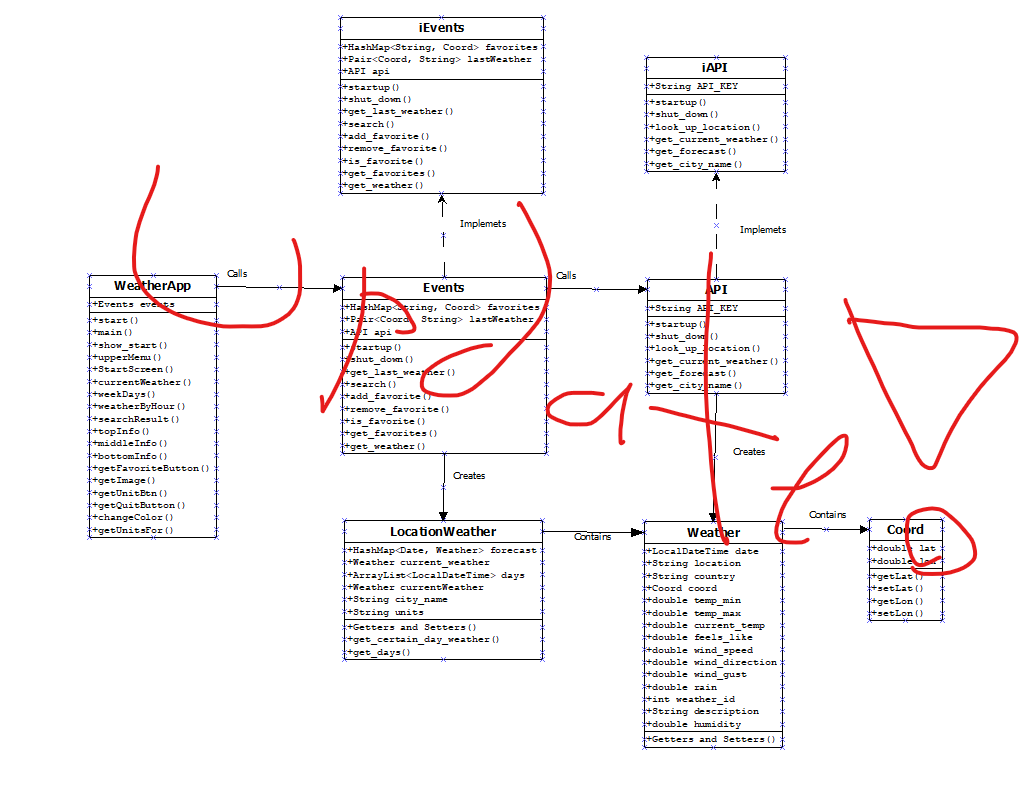
\includegraphics[width=0.3\textwidth]{class_diagram.png}
    \caption{UML Class Diagram of WeatherApp}
    \label{fig:class_diagram}
\end{figure}

\FloatBarrier

\subsection{Class Responsibilities}

Provide a brief description of the responsibilities of key classes identified in the class diagram.

\section{Project Functionality}

Describe the main functionality of the WeatherApp, including any extra features. Use clear and concise language.

\section{Implemented Classes}

List and briefly describe classes implemented by the team, specifying pre and post conditions where applicable.

\section{Division of Work}

Provide details on how the work was divided among team members, both agreed and actual.

\section{User Manual}

This section gives a brief introduction into using the WeatherApp program.

\subsection{Running}


\section{Known Bugs and Missing Features}

Document any known bugs or features that are yet to be implemented.

\section{Conclusion}

Summarize the key points covered in the document.

\end{document}
